\documentclass{article}

% Use the Cactus ThornGuide style file
% (Automatically used from Cactus distribution, if you have a 
%  thorn without the Cactus Flesh download this from the Cactus
%  home page at www.cactuscode.org)
\usepackage{../../../../doc/latex/cactus}

\begin{document}

\title{IOUtil}
\author{Thomas Radke, Gabrielle Allen}
\date{$ $Date$ $}

\maketitle

% Do not delete next line
% START CACTUS THORNGUIDE

\section{Introduction}

This document details the thorns provided in the standard Cactus distribution
for the output of grid variables, and describes how to set parameters for I/O
and checkpointing/recovery using these thorns.

Input and output of data (I/O) in Cactus is provided by infrastructure thorns,
which interact with the flesh via a fixed interface, which is described in the
Users' Guide. The standard release of Cactus contains a number of thorns which
provide so-called I/O methods implementing the actual I/O in a variety of data
formats and styles. All these provided I/O methods use thorn {\bf IOUtil} which
provides general utilities for I/O (such as parsing
parameter strings to decide which variables to output), and a general set of
parameters which are inherited by the different I/O methods (such as the output
directory). Thorn {\bf IOUtil} by itself provides no I/O methods.

More information about I/O and visualisation of Cactus data can be found in the
individual I/O thorns, and in the {\tt Visualization-HOWTO} available on the
Cactus web pages.

\section{I/O Methods in Cactus}

Cactus has several I/O methods for the output of grid variables in different
data formats and styles. Each I/O method comes with its own parameters by which
it can be customised, and all methods are registered with the flesh, satisfying
the Cactus API, allowing them to be called directly from application thorns.
An I/O method registers itself with the flesh along with it's name, and these
registered names are the labels we now use to describe the various methods.


\begin{table}
\begin{center}
\begin{tabular}{|l|l|l|}
  \hline
  {\bf I/O method} & {\bf Description} & {\bf Providing Thorn}\\
  \hline
  {\tt Scalar} &
  output of scalars or grid array reductions in xgraph or gnuplot format &
  {\tt CactusBase/IOBasic}
\\
  {\tt Info}      &
  screen output of scalars or grid array reductions &
  {\tt CactusBase/IOBasic}
\\
&&\\
  {\tt IOASCII\_1D} &
  1D line output of grid arrays in xgraph or gnuplot format &
  {\tt CactusBase/IOASCII}
\\
  {\tt IOASCII\_2D} &
  2D slice output of grid arrays in gnuplot format &
  {\tt CactusBase/IOASCII}
\\
  {\tt IOASCII\_3D} &
  full output of 3D grid arrays in gnuplot format &
  {\tt CactusBase/IOASCII}
\\
&&\\
  {\tt IOJpeg} &
  2D slice output of grid arrays in jpeg image format &
  {\tt CactusIO/IOJpeg}
\\
&&\\
  {\tt IOHDF5} &
  full output of arbitrary grid variables in HDF5 format &
  {\tt CactusPUGHIO/IOHDF5}
\\
&&\\
  {\tt IOFlexIO\_2D} &
  2D slice output of grid arrays in FlexIO format &
  {\tt CactusPUGHIO/IOFlexIO}
\\
  {\tt IOFlexIO} &
  full output of arbitrary grid variables in FlexIO format &
  {\tt CactusPUGHIO/IOFlexIO}
\\
  \hline
\end{tabular}
\caption{Standard I/O methods provided with the Cactus distribution}
\label{one}
\end{center}
\end{table}

The standard provided Cactus I/O methods are shown in Table~\ref{one}.
As described above, each of these I/O thorns inherit parameters from thorn
{\bf IOUtil}, which must be included in your ThornList
and activated in your parameter files before any of these I/O methods
can be used. {\bf IOUtil} allows you to set the default
behaviour for all the I/O methods described above, for example, setting
the parameter {\tt IO::out\_every = 1} will result in any chosen I/O method
providing output on each iteration. The default behaviour can be overridden
by specific parameters for each method.
For example, you may want scalar and 1D output at every iteration
but computationally expensive 3D output only every 10th iteration,
with these files going into another directory on a scratch partition.


\section{Providing Your Own I/O Method}

If you as a Cactus developer have your own input/output routines and want to
share this functionality with other people you should do this by putting them
into an new I/O thorn and register them as an I/O method.
A description on how to register a new I/O method with the flesh's I/O subsystem
can be found in the {\it Infrastructure Thorn Writer's Guide} (as part of the
{\it Cactus User's Guide}).

New I/O thorns should always inherit from thorn {\bf IOUtil} in order
to reuse as much of the existing I/O infrastructure as possible, and to maintain
a uniform interface on how to use the I/O methods.


%\section{External Packages}
%
%NOTE: This section will not be filled out properly until the new treatment of external
%packages is implemented.
%
%Some of the I/O methods used by Cactus require that external packages are installed and available
%on your machine.
%
%\begin{itemize}
%
%\item{\tt HDF5} {\bf Hierarchical Data Format}\\
%{\tt http://hdf.ncsa.uiuc.edu/}
%
%\item{\tt IEEEIO} \\
%{\tt http://zeus.ncsa.uiuc.edu/}
%
%\end{itemize}

\section{Standard Parameters}

Here we describe a few of the standard parameters used by {\bf IOUtil} to
control output.
\begin{itemize}

  \item{\tt IO::out\_dir}\\
    The name of the directory to be used for output. All the I/O methods
    described here will write by default to this directory (which itself
    defaults to the current working directory). Individual methods have
    parameters which can direct their output to a different directory.

  \item{\tt IO::out\_criterion}\\
    The criterion that decides when to output.  The default is to
    output every so many iterations (see {\tt IO::out\_every}).

  \item{\tt IO::out\_every}\\
    How often, in terms of iterations, each of the Cactus I/O methods
    will write
    output. Again, individual methods can set their own parameters to override
    this. The default is to never write output.

  \item{\tt IO::out\_dt}\\
    How often, in terms of simulation time, each of the Cactus I/O
    methods will write output.  Again, individual methods can set
    their own parameters to override this.  The default is to never
    write output.
\end{itemize}


\section{Saving/Generating Parameter Files}

Thorn {\bf IOUtil} can save a copy of the parameter file of a run, or can also
automatically generate a parameter file from all current parameter settings.
This is controlled by the {\tt IO::parfile\_write} parameter:

\begin{itemize}

  \item{\tt IO::parfile\_write="copy"}\\
    This is the default option, and makes an exact replica of the input
    parameter file in the standard output directory (this is particularly useful
    when the output directory is going to be archived).

  \item{\tt IO::parfile\_write="generate"}\\
    Generate a new parameter file from runtime information, containing the
    Cactus version, the name of the original parameter file, the run time/date,
    the host to run on, and the number of processors -- all on comment lines.
    Following this the parameter file contains the ActiveThorns list plus a
    sorted list of all active thorns' parameters which have been set in the
    original parameter file.

  \item{\tt IO::parfile\_write="no"}\\
    Switch off writing of a new parameter file.

\end{itemize}

The name of the new parameter file defaults to the original filename, unless the
parameter {\tt IO::parfile\_name} is set. Note that an already existing file
with the chosen name will be overwritten unless it is identical with the
original parameter file, or if Cactus was recovered from a checkpoint (in which
case you don't want to overwrite an existing parameter file with your recovery
parameter file).


\section{I/O Modes}
\label{iomodes}
For a run on multiple processors, scalar, 1D, and 2D output will always be
written from only processor zero (that is, required data from all other
processors will be sent to processor zero, which then outputs all the gathered
data). For full-dimensional output of grid arrays this may become a quite expensive
operation since output by only a single processor will probably result in an
I/O bottleneck and delay further computation. For this reason Cactus offers
different I/O modes for such output which can be controlled by the
{\tt IO::out\_mode} parameter, in combination with {\tt IO::out\_unchunked}
and {\tt IO::out\_proc\_every}. These parameters allow I/O to be optimised for
your particular machine architecture and needs:

\begin{itemize}
  \item {\tt IO::out\_mode = "onefile"}\\
    As for the 1D and 2D I/O methods, writing to file is performed only
    by processor zero.
    This processor gathers all the output data from the other processors
    and then writes to a single file. The gathered grid array data from each
    processor can be either written in chunks ({\tt IO::out\_unchunked =
    "no"}) with each chunk containing the data from a single processor, or
    collected into a single global array before writing ({\tt
    IO::out\_unchunked = "yes"}). The default is to write the data in chunks.
    This can be changed by adding an option string to the group/variable name(s)
    in the {\tt out\_vars} parameter with the key {\tt out\_unchunked} and an
    associated string value {\tt "yes|no|true|false"}.

  \item {\tt IO::out\_mode = "np"}\\
    Output is written in parallel for groups of processors. Each group
    consists of {\tt IO::out\_proc\_every} processors which have assigned one I/O
    processor which gathers data from the group and writes it to file. The
    chunked output will go into {\tt IO::out\_proc\_every} files.
    The default number of processors in a group is eight.

  \item {\tt IO::out\_mode = "proc"}\\
    This is the default output mode.
    Every processor writes its own chunk of data into a separate output file.
\end{itemize}

Probably the single-processor {\tt "proc"} mode is the most efficient output
mode on machines with a fast I/O subsystem and many I/O nodes (e.g. a Linux
cluster with local disks attached to each node) because it provides the highest
parallelity for outputting data. Note that on very large numbers of processors
you may have to fall back to {\tt "np"}, doing output by every so many processors,
mode if the system limit of maximum open file descriptors is exceeded (this is
true for large jobs on a T3E).

While the {\tt "np"} and {\tt "proc"} I/O modes are fast for outputting large
amounts of data from all or a group of processors in parallel, they have
the disadvantage of writing chunked files. These files then have to be
recombined during a postprocessing phase so that the final unchunked data can be
visualized by standard tools. For that purpose a recombiner utility program is
provided by the thorns offering parallel I/O methods.


\section{Output of Hyperslab Data}

While some I/O methods ({\tt IOHDF5, IOFlexIO}) can dump the full
contents of a multidimensional CCTK variable, others such as {\tt IOASCII\_1D}
and {\tt IOASCII\_2D} will output only a subset of the data (e.g. 1D lines or 2D
planes of 3D grid functions).
Such a subset (called a {\it hyperslab}) is generally defined as an orthogonal
region into the multidimensional dataset, with a start point and a length in any
direction, and an optional downsampling factor.

Thorn {\bf IOUtil} defines a set of hyperslab parameters for all
I/O methods which determine the default positions of 1D line or 2D slice output
along the axes. I/O thorns can also define their own hyperslab parameters
which then will overwrite the defaults provided by {\bf IOUtil}.

\begin{itemize}
  \item {\tt IO::out\_[xyz]line\_[xyz]}\\
    specifies the slice center for 1D x,y,z-line output by coordinate values
    of the underlying physical grid
  \item {\tt IO::out\_[xyz]line\_[xyz]i}\\
    specifies the slice center of 1D x,y,z-line output by index points
    of the underlying computational grid
  \item {\tt IO::out\_[\{xy\}\{xz\}\{yz\}]plane\_[xyz]}\\
    specifies the slice center of 2D xy,xz,yz-plane output by coordinate values
    of the underlying physical grid
  \item {\tt IO::out\_[\{xy\}\{xz\}\{yz\}]plane\_[xyz]}i\\
    specifies the slice center of 2D xy,xz,yz-plane output by index points
    of the underlying computational grid
  \item {\tt IO::out\_downsample\_[xyz]}\\
    specifies the downsampling factor for output in every direction
\end{itemize}

Setting the index points for the slice centers in a parameter file has
precedence over setting their location by coordinate values.
If nothing was specified the default values of {\tt IO::out\_[xyz]line\_[xyz]}
and {\tt IO::out\_[\{xy\}\{xz\}\{yz\}]plane\_[xyz]} will be used.
These are set to be all zeros which causes the output to go through the
coordinate system's origin or the closest grid point to this (see figure
\ref{default_1D_output} for an example).

\begin{figure}[ht]
\begin{center}
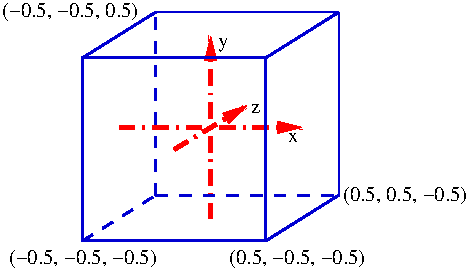
\includegraphics{1Dlines_in_box}
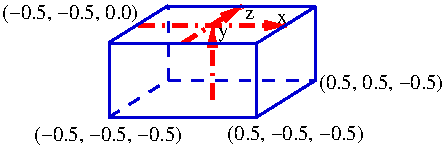
\includegraphics{1Dlines_in_xyBitant}
\end{center}
\caption{Default 1D {\it x,y,z}-line output for a 3D grid in box mode (left) and {\it xy}-bitant mode (right)}
\label{default_1D_output}
\end{figure}

If the coordinate values specified in {\tt IO::out\_[xyz]line\_[xyz]}
or {\tt IO::out\_[\{xy\}\{xz\}\{yz\}]plane\_[xyz]} lie outside the physical
grid, the slice center simply reverts to the center of the box in that
direction. This fallback method method can be changed to using 0-slices instead
by setting the corresponding {\tt IO::out\_[xyz]line\_[xyz]i}
and {\tt IO::out\_[\{xy\}\{xz\}\{yz\}]plane\_[xyz]i} parameter(s) to the value
{\tt -2}.

Although they are not hyperslabs by the above definition, output of 1D diagonals
for 3D grid arrays is also supported by I/O method {\tt IOASCII\_1D} but has the
restriction that the line will always start in the bottom-left corner of the
computational grid and steadily rise by one grid point in every direction (see
figure \ref{default_diagonal_output} for an example).

\begin{figure}[ht]
\begin{center}
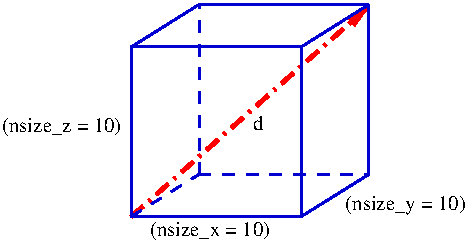
\includegraphics{diagonal_in_cubic}
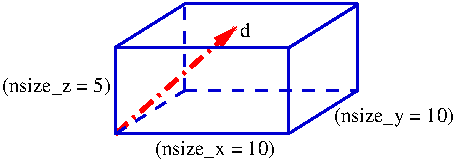
\includegraphics{diagonal_in_noncubic}
\end{center}
\caption{1D diagonal output for a 3D cubical (left) and non-cubical (right)
computational grid}
\label{default_diagonal_output}
\end{figure}


\section{Data Filenames}

The standard I/O thorns in Cactus make use of a consistent set of filenames
and extensions, which identify the variables and data format used in the file.
The filenames are listed in the following table.
%The filenames are listed in Table~\ref{filename_table},
%and the extensions in Table~\ref{filename_extensions_table}

\begin{table}[htb]
\begin{center}
\label{filename_table}
\begin{tabular}{|l|l|}
  \hline
  {\bf I/O method}   & {\bf Filename for output of variable {\tt var}}\\
  \hline
  {\tt Info}         & only outputs to screen\\
  {\tt Scalar}       & {\tt <var>.\{asc|xg\}} for scalar variables\\
                     & {\tt <var>\_<reduction>.\{asc|xg\}} for reduction values from grid arrays\\
  {\tt IOASCII\_1D}  & {\tt <var>\_<slice>\_[<center\_i>][center\_j>].\{asc|xg\}}\\
  {\tt IOASCII\_2D}  & {\tt <var>\_<plane>\_[<center>].asc}\\
  {\tt IOASCII\_3D}  & {\tt <var>\_3D.asc}\\
  {\tt IOJpeg}       & {\tt <var>\_<plane>\_[<center>].jpeg}\\
  {\tt IOHDF5}       & {\tt <var>\_3D.h5}\\
  {\tt IOFlexIO\_2D} & {\tt <var>\_2D.ieee}\\
  {\tt IOFlexIO}     & {\tt <var>\_3D.ieee}\\
  \hline
\end{tabular}
\caption{Filenames used by standard I/O thorns}
\end{center}
\end{table}

%\begin{table}[htb]
%\begin{center}
%\label{filename_extensions_table}
%\begin{tabular}{|c|l|l|}
%\hline
%{\bf Extension} & {\bf Description} & {\bf Thorn} \\
%  \hline
% {\tt .xl} & 1D line plots in {\it x}-direction & {\tt CactusBase/IOASCII}\\
% {\tt .yl} & 1D line plots in {\it y}-direction & {\tt CactusBase/IOASCII}\\
% {\tt .zl} & 1D line plots in {\it z}-direction & {\tt CactusBase/IOASCII}\\
% {\tt .dl} & 1D diagonal line plots             & {\tt CactusBase/IOASCII}\\
% {\tt .tl} & traceline plots over time          & {\tt CactusBase/IOBasic}\\
%  \hline
%\end{tabular}
%\caption{File extensions used by the standard I/O thorns}
%\end{center}
%\end{table}


\section{Checkpointing and Recovery in Cactus}
\label{cp_recovery}

The I/O methods for arbitrary output of CCTK variables also provide functionality for {\it checkpointing}
and {\it recovery}. A checkpoint is a snapshot of the current state of the
simulation ({\it i.e.} the contents of all the grid variables and the parameter
settings) at a chosen timestep. Each checkpoint is saved into a
{\it checkpoint file} which can be used to restart a new simulation at a later
time, recreating the exact state at which it was checkpointed.

Checkpointing is especially useful when running Cactus in batch queue systems
where jobs get only limited CPU time. A more advanced use of checkpointing
would be to restart your simulation after a crash or a problem had developed,
using a  different parameter set recovering from the latest stable timestep.
Additionally, for performing parameter studies,  compute-intensive
initial data can be calculated just once and saved in a checkpoint file
from which each job can be started.

Again, thorn {\bf IOUtil} provides general checkpoint \& recovery
parameters. The most important ones are:
\begin{itemize}
  \item {\tt IO::checkpoint\_every} (steerable)\\
    specifies how often to write a evolution checkpoint in terms of iteration
    number.
  \item {\tt IO::checkpoint\_every\_walltime\_hours} (steerable)\\
    specifies how often to write a evolution checkpoint in terms of
    wall time.  Checkpointing will be triggered if either of these
    conditions is met.
  \item {\tt IO::checkpoint\_next} (steerable)\\
    triggers a checkpoint at the end of the current iteration.  This
    flag will be reset afterwards.
  \item {\tt IO::checkpoint\_ID}\\
    triggers a checkpoint of initial data
  \item {\tt IO::checkpoint\_on\_terminate} (steerable)\\
    triggers a checkpoint at the end of the last iteration of a simulation run
  \item {\tt IO::checkpoint\_file} (steerable)\\
    holds the basename for evolution checkpoint file(s) to create\\
    Iteration number and file extension are appended by the individual I/O
    method used to write the checkpoint.
  \item {\tt IO::checkpoint\_ID\_file} (steerable)\\
    holds the basename for initial data checkpoint file(s) to create\\
    Iteration number and file extension are appended by the individual I/O
    method used to write the checkpoint.
  \item {\tt IO::checkpoint\_dir}\\
    names the directory where checkpoint files are stored
  \item {\tt IO::checkpoint\_keep} (steerable)\\
    specifies how many evolution checkpoints should be kept\\
    The default value of $1$ means that only the latest evolution checkpoint
    is kept and older checkpoints are removed in order to save disk space.
    Setting {\tt IO::checkpoint\_keep} to a positive value will keep so many
    evolution checkpoints around. A value of $-1$ will keep all (future) checkpoints.
  \item {\tt IO::recover\_and\_remove}\\
    determines whether the checkpoint file that the current simulation has
    been successfully recovered from, should also be subject of removal,
    according to the setting of {\tt IO::checkpoint\_keep}
  \item {\tt IO::recover}\\
    keyword parameter telling if/how to recover.\\
    Choices are {\tt "no"}, {\tt "manual"}, {\tt "auto"}, and {\tt "autoprobe"}.
  \item {\tt IO::recover\_file}\\
    basename of the recovery file\\
    Iteration number and file extension are appended by the individual I/O
    method used to recover from the recovery file.
  \item {\tt IO::recover\_dir}\\
    directory where the recovery file is located
  \item {\tt IO::truncate\_files\_after\_recovering}\\
    whether or not to truncate already existing output files after recovering
\end{itemize}

To checkpoint your simulation, you need to enable checkpointing by setting
the boolean parameter {\tt checkpoint}, for one of the appropriate I/O methods to
{\tt yes}.
Checkpoint filenames consist of a basename (as specified in {\tt
IO::checkpoint\_file}) followed by {\tt ".chkpt.it\_$<$iteration\_number$>$"}
plus the file extension indicating the file format ({\tt "*.ieee"} for IEEEIO
data from {\tt CactusPUGHIO/IOFlexIO}, or {\tt "*.h5"} for HDF5 data from
{\tt CactusPUGHIO/IOHDF5}).

Use the {\tt "manual"} mode to recover from a specific checkpoint file by adding
the iteration number to the basename parameter.

The {\tt "auto"} recovery mode will automatically recover from the latest
checkpoint file found in the recovery directory.
In this case {\tt IO::recover\_file} should contain the basename only (without
any iteration number).

The {\tt "autoprobe"} recovery mode is similar to the {\tt "auto"} mode except
that it would not stop the code if no checkpoint file was found but only print
a warning message and then continue with the simulation. This mode allows you
to enable checkpointing and recovery in the same parameter file and use that
without any changes to restart your simulation. On the other hand, you are
responsible now for making the checkpoint/recovery directory/file parameters
match --- a mismatch will not be detected by Cactus in order to terminate it.
Instead the simulation would always start from initial data without any
recovery.

Because the same I/O methods implement both output of arbitrary data and checkpoint
files, the same I/O modes are used (see Section~\ref{iomodes}).
Note that the recovery routines in Cactus can process both chunked and unchunked
checkpoint files if you restart on the same number of processors --- no
recombination is needed here. That's why you should always use one of the
parallel I/O modes for checkpointing. If you want to restart on a different
number of processors, you first need to recombine the data in the checkpoint
file(s) to create a single file with unchunked data.
Note that Cactus checkpoint files are platform independent so you can restart
from your checkpoint file on a different machine/architecture.

By default, existing output files will be appended to rather than truncated after
successful recovery. If you don't want this, you can force I/O methods to
always truncate existing output files. Thorn {\bf IOUtil} provides an aliased
function for other I/O thorns to call:
\begin{verbatim}
  CCTK_INT FUNCTION IO_TruncateOutputFiles (CCTK_POINTER_TO_CONST IN cctkGH)
\end{verbatim}
This function simply returns 1 or 0 if output files should or should not be truncated.

\vskip .5cm
\noindent{\bf WARNING:}

\noindent
Checkpointing and recovery should {\bf always} be tested for a new thorn set.
This is because only Cactus grid variables and parameters are saved in a
checkpoint file. If a thorn has made use of saved local variables, the state of
a recovered simulation may differ from the original run. To test checkpointing
and recovery, simply perform one run of say 10 timesteps, and compare output
data with a checkpointed and recovered run at say the 5th timestep.
The output data should match exactly if recovery was successful.


\section{Reading Data from Files into Cactus}

The very same routines which implement checkpointing/recovery functionality
in the {\tt IOHDF5} and {\tt IOFlexIO} thorns are also used to provide
file reader capabilities within Cactus. They enable users to read variables,
whose contents were written to files in HDF5 or IEEEIO data format, back into
Cactus at a later time. This is especially useful if compute-intensive
initial data is calculated only once and stored in a file. Such data
can then be read back in at startup and immediately used by following evolution
runs.

The following {\bf IOUtil} parameters exist to specify what variables should be
read from file(s) as initial data:

\begin{itemize}
  \item {\tt IO::filereader\_ID\_dir}\\
    root directory for files to be read
  \item {\tt IO::filereader\_ID\_files}\\
    list of files to read in as initial data (multiple filenames must be
    separated by spaces)\\
    The same file naming conventions (what I/O mode used, which iteration
    number) apply as for checkpoint files.
  \item {\tt IO::filereader\_ID\_vars}\\
    list of CCTK variables to read in from the given initial data files
    (variables are identified by their full name, multiple variable names must
    be separated by spaces)\\
    This is useful if a datafile contains multiple variables but only some of
    them should be read. Thus it is possible to recover distinguished variables
    from a full checkpoint file.\\
    Note that if the file contains several timesteps of the same variable only
    the last one is taken by default. This can be changed by adding an option
    string with the key {\tt cctk\_iteration} and an associated integer scalar
    value to the variable name denoting the iteration number to choose, like in
    {\tt IO::filereader\_ID\_vars = "wavetoy::phi\{ cctk\_iteration = 10 \}"}.
    The file reader supports a further option {\tt alias} and an associated
    string scalar value which can be used to set the dataset in the initial
    data files that will be read into this variable. For example {\tt
    IO::filereader\_ID\_vars = "wavetoy::phi\{ alias='wavetoy::psi' \}"} will
    read the data of variable {\tt wavetoy::psi} from file into 
    {\tt wavetoy::phi}. This option requires that explicit variable names are
    used, group names are not supported for the {\tt alias} option.
\end{itemize}

Thorn {\bf IOUtil} also provides a filereader API which can be called
by any application thorn at any time. It gets passed the equivalent information
to the filereader parameters, plus a pointer to the underlying CCTK grid
hierarchy. The return code denotes the total number of variables recovered by
the filereader.

C API:
\begin{verbatim}
  #include "CactusBase/IOUtil/src/ioutil_CheckpointRecovery.h"


  int IOUtil_RecoverVarsFromDatafiles (cGH *GH,
                                       const char *in_files,
                                       const char *in_vars);
\end{verbatim}

Fortran API:
\begin{verbatim}
  call IOUtil_RecoverVarsFromDatafiles (result, GH, in_files, in_vars)

    integer       result
    CCTK_POINTER  GH
    character*(*) in_files
    character*(*) in_vars
\end{verbatim}

If data is to be imported from files which were not created by {\tt IOHDF5} or
{\tt IOFlexIO} it needs to be converted first into the appropriate HDF5 or
IEEEIO file format and the file layout which either one of these thorns uses.
This is described in detail in the thorns' documentation, along with a simple C
source file which can be used as a template to build your own data converter
program.


\section{Example Parameter Files}

Here we give examples of the parameters for the different I/O methods.

\begin{itemize}
\item{\bf Output information to screen using {\tt IOBasic's "Info"}} I/O method
\begin{verbatim}
  ActiveThorns = "IOBasic IOUtil PUGHReduce ..."

  # Output using all methods on iteration 0, 10, 20, ...
  IO::out_every = 10

  # Group of variables to output to screen
  IOBasic::outInfo_vars = "evolve::vars"
\end{verbatim}

\item{\bf Scalar Output from {\tt IOBasic's "Scalar"} I/O method}
\begin{verbatim}
  ActiveThorns = "IOBasic IOUtil PUGHReduce ..."

  # Output vars using scalar method on iteration 0, 10, 20, ...
  IOBasic::outScalar_every = 10

  # Group of variables to output to file
  IOBasic::outScalar_vars = "evolve::vars"
\end{verbatim}

\item{\bf ASCII 1D and 2D Output with {\tt IOASCII's "IOASCII\_1D"} and
{\tt "IOASCII\_2D"} I/O methods}
\begin{verbatim}
  ActiveThorns = "IOASCII IOUtil PUGHSlab ..."

  # Output vars in 1D on iteration 0, 10, 20, ...
  IOASCII::out1D_every = 10

  # Output vars in 2D on iteration 0, 50, 100, ...
  IOASCII::out2D_every = 50
\end{verbatim}

\item{\bf HDF5 Output with {\tt IOHDF5's "IOHDF5"} I/O method}
\begin{verbatim}
  ActiveThorns = "IOHDF5 IOUtil PUGHSlab ..."

  # Output vars in HDF5 format on iteration 0, 5, 10, ...
  IOHDF5::out_every = 5

  # Group of variables to output
  IOHDF5::out_vars = "evolve::vars"

  # Special I/O directory for HDF5 output
  IOHDF5::out_dir = "/scratch/tmp"

  # Full output unchunked to one file
  # (Only using a small number of processors)
  IO::out_mode      = "onefile"
  IO::out_unchunked = "yes"

  # Downsample full data by a factor of 3 in each direction
  IO::out_downsample_x = 3
  IO::out_downsample_y = 3
  IO::out_downsample_z = 3
\end{verbatim}

\item{\bf IEEEIO 2D hyperslab and full output using {\tt IOFlexIO's "IOFlexIO\_2D"} and {\tt "IOFlexIO"} I/O methods}
\begin{verbatim}
  ActiveThorns = "IOFlexIO FlexIO IOUtil PUGHSlab ..."

  # Output vars in 2D IEEEIO format on iteration 0, 100, 200, ...
  IOFlexIO::out2D_every = 100

  # Output vars in IEEEIO format on iteration 0, 5, 10, ...
  IOFlexIO::out_every = 5

  # Group of variables to output to file for each method
  IOFlexIO::out2D_vars = "evolve::vars"
  IOFlexIO::out_vars   = "evolve::vars"

  # 2D output goes into standard I/O directory
  IO::out_dir = "test"

  # Special I/O directory for full output
  IOFlexIO::out_dir = "/scratch/tmp"

  # Full output chunked to one file for every eight processors
  # (Run on large number of processors)
  IO::out_mode       = "np"
  IO::out_proc_every = 8
  IO::out_unchunked  = "no"

  # Downsample full data by a factor of 3 in each direction
  IO::out_downsample_x = 3
  IO::out_downsample_y = 3
  IO::out_downsample_z = 3
\end{verbatim}

\item{\bf Checkpointing using thorn {\tt IOFlexIO}}
\begin{verbatim}
  ActiveThorns = "IOFlexIO FlexIO IOUtil PUGHSlab ..."

  # Use IEEEIO data format for checkpoint files
  IOFlexIO::checkpoint = "yes"

  # Make a new checkpoint file every 300 iterations
  IO::checkpoint_every = 300

  # Name and directory of checkpoint file
  IO::checkpoint_file = "run5"
  IO::checkpoint_dir  = "/scratch/tmp"
\end{verbatim}

\item{\bf Recovering from a checkpoint file}
\begin{verbatim}
  ActiveThorns = "IOFlexIO FlexIO IOUtil PUGHSlab ..."

  # automatically choose the latest checkpoint file
  IO::recover = "auto"

  # Name and directory of checkpoint file to recover from
  IO::recover_file = "run5"
  IO::recover_dir  = "/scratch/tmp"
\end{verbatim}

\end{itemize}


\section{Providing Your own Checkpointing/Recovery Method}

This section is for Cactus developers to describe how they can add a new method
for checkpointing/recovery using the existing I/O parameters and the function
API of thorn {\bf IOUtil}.
Inheriting this functionality from thorn {\bf IOUtil} helps you to reuse
existing code and maintain a uniform user interface on how to invoke different
checkpointing/recovery methods.

\subsection{Adding a Checkpointing Method}

Checkpointing is similar to performing full output of an individual grid
variable, except that

\begin{enumerate}
  \item the output is done for all grid variables existing in a grid hierarchy
  \item in addition to the contents of all variables, also the current setting
    of all parameters is saved as well as some other information necessary for
    recovering from the checkpoint at a later time
\end{enumerate}

A thorn routine providing this checkpointing capability should register itself
with the flesh's scheduler at the {\tt CPINITIAL} (for initial data
checkpoints), {\tt CHECKPOINT} (for periodic checkpoints of evolution
data), and {\tt TERMINATE} time bins (for checkpointing the last timestep
of a simulation).

It should also decide whether checkpointing is needed by evaluating the
corresponding checkpoint parameters of {\bf IOUtil} (see section
\ref{cp_recovery}).

Before dumping the contents of a distributed grid array into a checkpoint
file the variable should be synchronized in case synchronization was not done before
implicitly by the scheduler.

To gather the current parameter values you can use the C routine
\begin{verbatim}
  char *IOUtil_GetAllParameters (const cGH *GH, int all);
\end{verbatim}
from thorn {\bf IOUtil}. This routine returns the parameter settings in an
allocated single large string. Its second argument {\tt all} flags whether all
parameter settings should be gathered ($!= 0$) or just the ones which have been
set before ($== 0$). Note that you should always save all parameters in a
checkpoint in order to reproduce the same state after recovery.

As additional data necessary for proper recovery, the following information
must be saved in a checkpoint file:
\begin{itemize}
  \item the current main loop index (used by the driver as the main evolution
    loop index)
  \item the current CCTK iteration number ({\tt GH->cctk\_iteration})
  \item the physical simulation time ({\tt GH->cctk\_time})
\end{itemize}

Moreover, information about the I/O mode used to create the checkpoint
(chunked/unchunked, serial versus parallel I/O), the active thorns list, or
this run's Cactus version ID (for compatibility checking at recovery time) could
be relevant to save in a checkpoint.


\subsection{Adding a Recovery Method}

Recovering from a checkpoint is a two step operation:
\begin{enumerate}
  \item Right after reading the parameter file and finding out if recovery was
    requested, all the parameters are restored from the checkpoint file
    (overwriting any previous settings for non-steerable parameters).
  \item After the flesh has created the grid hierarchy with all containing grid
    variables and the driver has set up storage for these, their contents is
    restored from the checkpoint (overwriting any previously initialized
    contents).
\end{enumerate}

The flesh provides the special time bins {\tt RECOVER\_PARAMETERS} and
{\tt RECOVER\_VARIABLES} for these two steps (see also the chapter on
{\it Adding a Checkpointing/Recovery Method} in the {\it Infrastructure Thorn
Writer's Guide} as part of the {\it Cactus User's Guide}).\\

Thorn {\bf IOUtil} evaluates the recovery parameters (determines the recovery
mode to use, construct the name(s) of the recovery file(s) etc.).
It also controls the recovery process by invoking the recovery methods of
other I/O thorns, one after another until one method succeeded.\\

A recovery method must provide a routine with the following prototype:

\begin{verbatim}
  int Recover (cGH *GH, const char *basefilename, int called_from);
\end{verbatim}

This routine will be invoked by {\bf IOUtil} with the following arguments:

\begin{itemize}
  \item a GH pointer refer to the grid hierarchy and its grid variables\\
    Note that this can also be a {\tt NULL} pointer if the routine was called
    at {\tt CP\_RECOVER\_PARAMETERS} when no grid hierarchy exists yet.

  \item the basename of the checkpoint file to recover from\\
    This name is constructed by {\bf IOUtil} from the settings of {\tt
    IO::recovery\_dir} and {\tt IO::recover\_file}. It will also include an
    iteration number if one of the {\tt auto} recovery modes is used.
    The filename extension by which checkpoint files of different recovery
    methods are distinguished must be appended explicitly.

  \item a flag identifying when the routine was called\\
    This can be one of the keywords {\tt CP\_INITIAL\_DATA, CP\_EVOLUTION\_DATA,
    CP\_RECOVER\_PARAMETERS, CP\_RECOVER\_DATA}, or {\tt FILEREADER\_DATA}).
    This flag tells the routine what it should do when it is being called by
    {\bf IOUtil}. Note that {\bf IOUtil} assumes that the recovery method can
    also be used as a filereader routine here which is essentially the same
    as recovering (individual) grid variables from (data) files.
\end{itemize}


To perform the first step of recovery process, a recovery method must register
a routine with the flesh's scheduler at the {\tt RECOVER\_PARAMETERS}
time bin. This routine itself should call the {\bf IOUtil} API

\begin{verbatim}
  int IOUtil_RecoverParameters (int (*recover_fn) (cGH *GH,
                                                   const char *basefilename,
                                                   int called_from),
                                const char *file_extension,
                                const char *file_type)
\end{verbatim}

which will determine the recovery filename(s) and in turn invoke the actual
recovery method's routine as a callback function. The arguments to pass to this
routine are

\begin{itemize}
  \item a function pointer {\tt recover\_fn} as a reference to the recovery
    method's actual recovery routine (as described above)

  \item {\tt file\_extension} -- the filename extension for recovery files
    which are accepted by this recovery method\\
    When {\bf IOUtil} constructs the recovery filename and searches for
    potential recovery files (in the {\tt auto} recovery modes) it will only
    match filenames with the basename as given in the {\tt IO::recovery\_file}
    parameter, appended by {\tt file\_extension}.

  \item {\tt file\_type} -- the type of checkpoint files which are accepted by
    this recovery method\\
    This is just a descriptive string to print some info output during recovery.
\end{itemize}

The routine registered at {\tt RECOVER\_PARAMETERS} should return to
the scheduler a negative value if parameter recovery failed for this recovery
method for some reason (e.g. if no appropriate recovery file was found).
The scheduler will then continue with the next recovery method until one
finally succeeds (a positive value is returned). If none of the available
recovery methods were successful the flesh would stop the code.

A value of zero should be returned to the scheduler to indicate that no
recovery was requested.\\

The second step during recovery --- restoring the contents of grid variables
from the recovery file --- is invoked by thorn {\bf IOUtil} which registers
a routine at {\tt RECOVER\_VARIABLES}. This routine calls all recovery
methods which were registered before with {\bf IOUtil} via the API

\begin{verbatim}
  int IOUtil_RegisterRecover (const char *name,
                              int (*recover_fn) (cGH *GH,
                                                 const char *basefilename,
                                                 int called_from));
\end{verbatim}

With this registration, all recovery method's actual recovery routines are made
known to {\bf IOUtil}, along with a descriptive name under which they are
registered.

At {\tt RECOVER\_VARIABLES} thorn {\bf IOUtil} will loop over all 
available recovery routines (passing the same arguments as for parameter
recovery) until one succeeds (returns a positive value).

% Do not delete next line
% END CACTUS THORNGUIDE

\end{document}
